\chapter{Coordinate Systems}
\label{app:coordinateSystems}
The geometries in the simulation are defined in their respective local coordinate systems $[x',y']$. Figure \ref{fig:localPosition2} shows an elliptical geometry defined in its local coordinate system about its origin. The local origin point is defined such that it is the center of rotation and any rotation will be prescribed about this point.

	\begin{figure}[h]
     \centering
     \begin{subfigure}[t]{0.45\textwidth}
             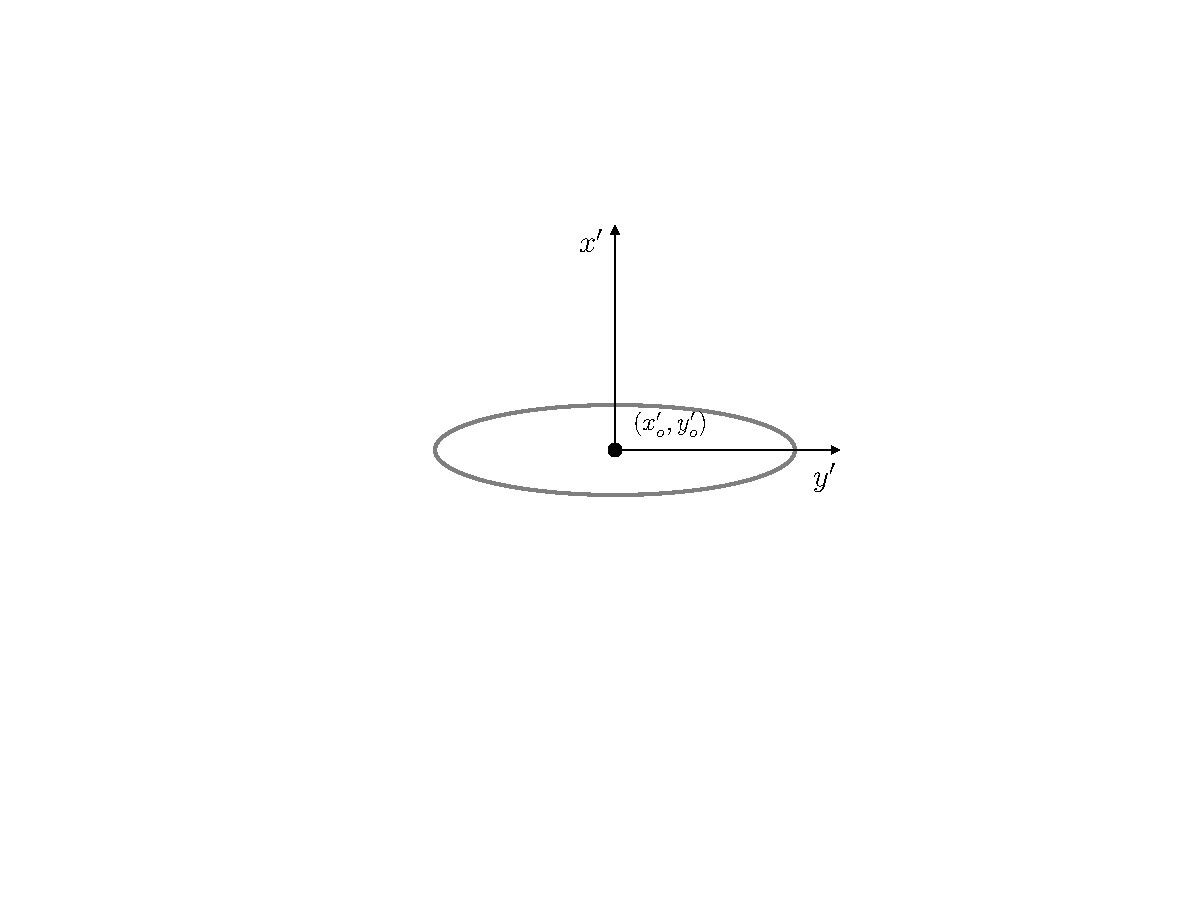
\includegraphics[trim=4.5cm 2.cm 3.5cm 1.5cm, clip, width=\linewidth]{./figures/coupling/interpolation/ellipse/localOrientation2.pdf}
             \caption{Local coordinate system $[x,y]'$}
             \label{fig:localPosition2}
     \end{subfigure}%
     ~ %add desired spacing between images, e. g. ~, \quad, \qquad etc.
       %(or a blank line to force the subfigure onto a new line)
     \begin{subfigure}[t]{0.45\textwidth}
             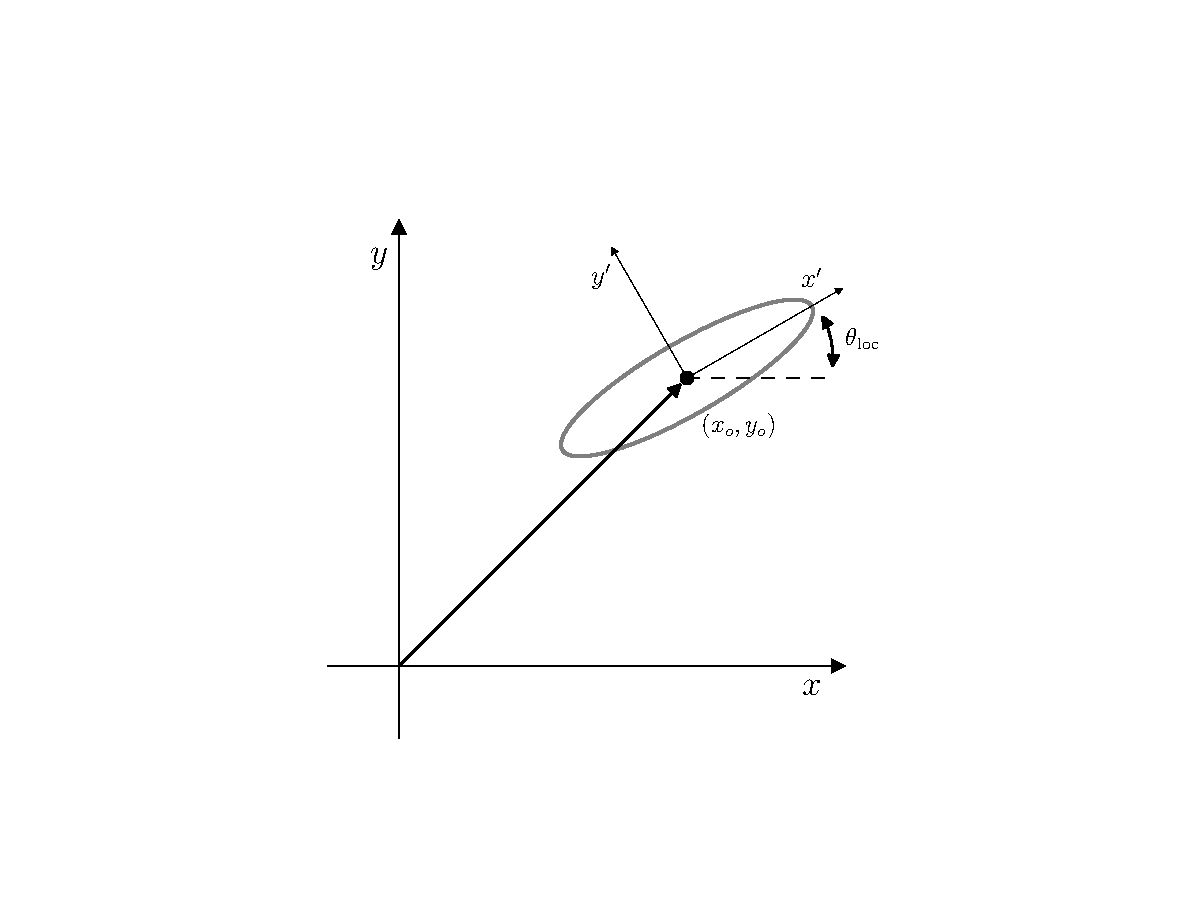
\includegraphics[trim=4.5cm 2.cm 3.5cm 1.5cm, clip, width=\linewidth]{./figures/coupling/interpolation/ellipse/globalOrientation.pdf}
             \caption{Global coordinate system $[x,y]$}
             \label{fig:globalPosition2}
     \end{subfigure}

     \caption{Ellipse defined in \textbf{(a)} the local coordinate system and \textbf{(b)} the global coordinate system. The geometry is positioned using the displacement vector $[x_o,y_o]$ and rotated by $\theta_0$ about the local origin point.}
     \label{fig:positionOfBody2}
	\end{figure}
	
The body is then transformed to the global coordinate system $[x,y]$ by the displacement vector $\mathbf{x}_o = [x_o,y_o]$ (i.e the global position of the local origin) and a local rotation by $\theta_{\mathrm{loc}}$ about the local origin $[x'_o,y'_o]$. The transformation of an arbitrary point $\mathbf{x}'_p = [x'_p,y'_p]$ in the local coordinate system to the global coordinate system is given as,

		\begin{equation}
		\mathbf{x}_p = 
		\begin{bmatrix}
		{x}_p\\
		{y}_p\\
		\end{bmatrix} = \begin{bmatrix}
		\cos\theta_{loc} & -\sin\theta_{loc}  \\
		\sin\theta_{loc}  & \cos\theta_{loc} 
		\end{bmatrix} \cdot \begin{bmatrix}
		x'_p-x'_o\\
		y'_p-y'_o\\
		\end{bmatrix} + 
		\begin{bmatrix}
		{x_{o}}\\
		{y_{o}}\\
		\end{bmatrix} 
		\end{equation}

where $\mathbf{x}_p = [x_p,y_p]$ is the global position of the point. The Eulerian solver defines the body mesh in the local coordinate system is then transformed to global position using these parameters. Similarly, the panel geometry for the Lagrangian solver is defined in the same fashion. For a moving bodies problem, the displacement vector and the local rotation angle can be updated to prescribe the motion.



%		\subsection{Coordinate Systems}
%			% Coordinate system: local to global transformation.
%			% summarize: coordinates systems of panels, lagrangian, eulerian
%			% how is the body defined? How it the problem constructed? 
